\documentclass[12pt]{article}
\usepackage{blindtext}
\usepackage[en,bordered]{uni-style}
\usepackage{uni-math}
\usepackage{subcaption}

\title{Sentiment Analysis and Stocks}
\prof{Dr. Khalaj}
\department{Department of Electrical Engineering}
\subtitle{Foundations of Data Science}
\subject{Project Report}
\info{
    \begin{tabular}{lr}
        Arad Mahdinejad Kashani & 400102028\\
    \end{tabular}
}
\date{\today}
\usepackage{uni-code}
\usepackage{graphicx}
\graphicspath{{pictures/}}
    
\begin{document}
\maketitlepage
\maketitlestart

\section{Introduction}
I did use Git for this project. I have messaged you on Telegram
so as to add you to my private repository. If needed, you can
contact my Telegram at \textit{@aradmnk}. Not much is happening, though.
There are only 4 python notebooks and the .csv file for the web-crawler
(`divar.csv', because I crawled `divar.ir').

The process is also documented in the notebook files themselves. 
There is text, and the code is segmented by the tasks in each 
phase of the project, so hopefully it is readable.

\pagebreak

\section{Phase 1}
After reading the files, I made a realization that there exists a
certain tag (referred to a \textbf{CashTag \$} in the paper mentioned
in the project documentation) in the df[`text'] column. I used regex
to separate them in a different column and used that from then on.

\subsection{Task 1}

\begin{qsolve}[Task]
    Find the most and least tweeted stocks.
\end{qsolve}

\begin{figure}[h!]
    \centering
    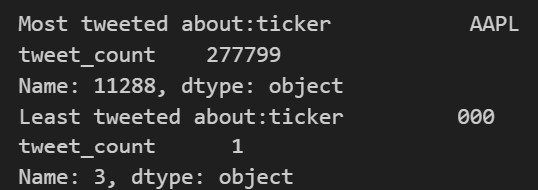
\includegraphics[width=.7\textwidth]{P1.1.jpg}
    \caption{Most and least stocks}
    \label{fig:1.1}
\end{figure}

As we can see, the most tweeted about stocks is \textbf{Apple Inc. \textit{(AAPL)}}.
The least tweeted about is irrelevant because there existed many tickers with
only 1 tweet (I checked it manually, it is not included in the notebook).

\begin{qsolve}[Task]
    Segment the companies based on tweet counts.
\end{qsolve}

\begin{figure}[h!]
    \centering
    \begin{subfigure}{.5\textwidth}
        \centering
        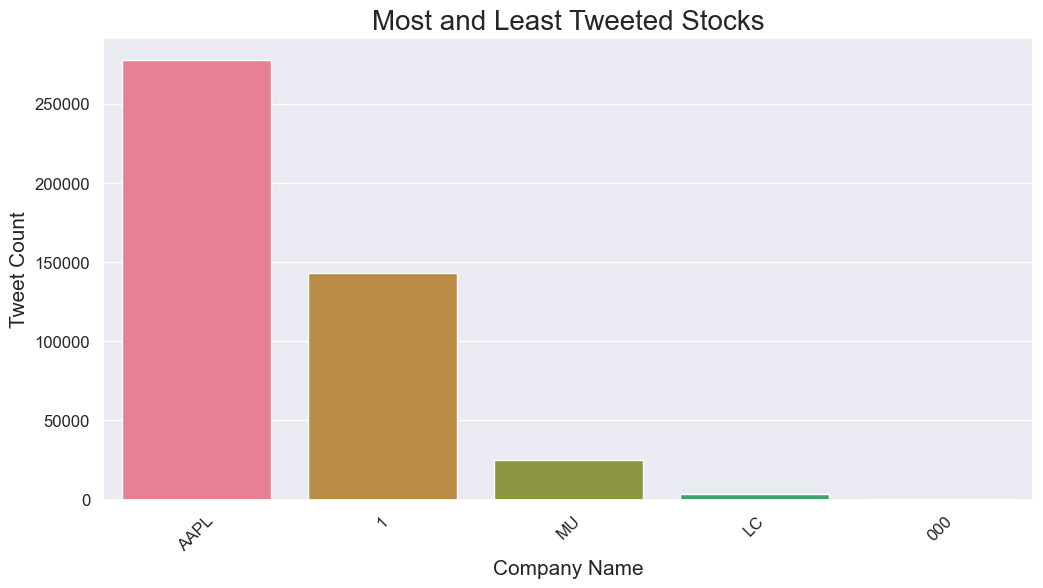
\includegraphics[width=.7\textwidth]{P1.1.2.png}
        \caption{Some companies and their respective tweet counts}
        \label{fig:1.1.2}
    \end{subfigure}%
    \begin{subfigure}{.5\textwidth}
        \centering
        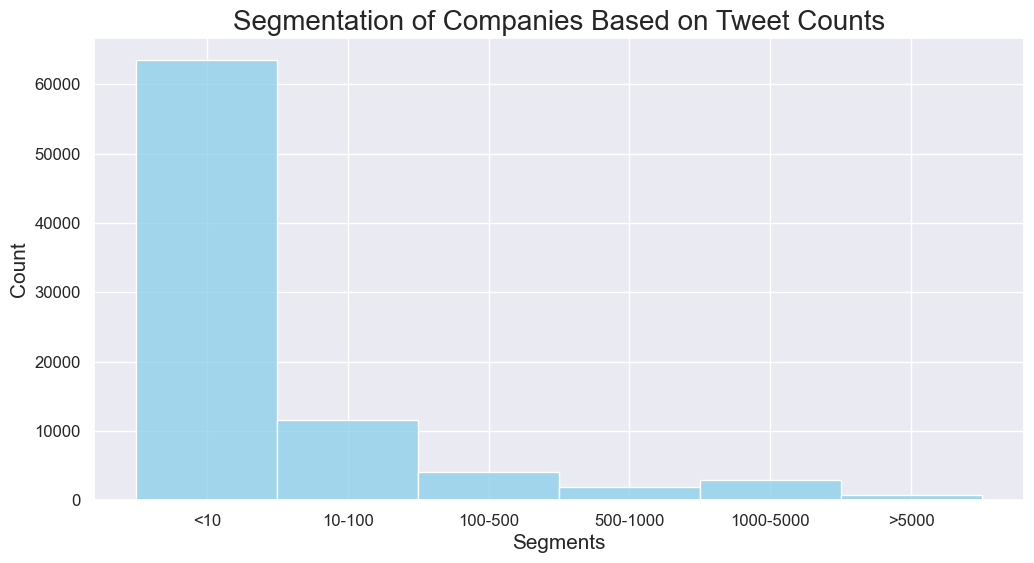
\includegraphics[width=.7\textwidth]{P1.1.3.png}
        \caption{Segmentation of the companies}
        \label{fig:1.1.3}
    \end{subfigure}
    \caption{}
\end{figure}

The middle companies of \textit{3.(a)} were 
hand picked from the middle, by index.

\pagebreak

\subsection{Task 2}

\begin{qsolve}[Task]
    Statistics on distributions of 5 individual 
    stocks over time. Choose the individual stocks to 
    perform reflect different sectors of the economy.
\end{qsolve}

\begin{figure}[h!]
    \centering
    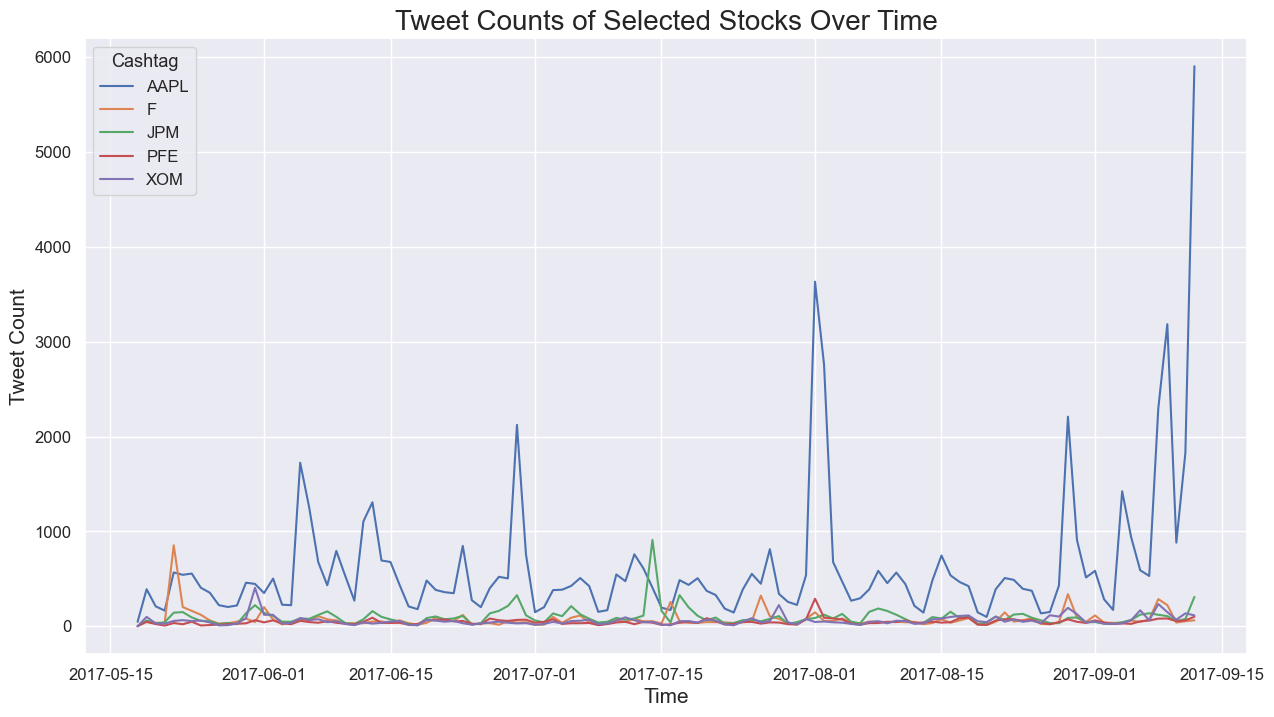
\includegraphics[width=1\textwidth]{P1.2.png}
    \caption{Individual stock distributions}
    \label{fig:1.2}
\end{figure}

I manually chose \textbf{Apple} (Technology), \textbf{ExxonMobil} (Energy), 
\textbf{Pfizer} (Healthcare), \textbf{JPMorgan Chase} (Financial), 
and \textbf{Ford} (Automotive).

\pagebreak

\subsection{Task 3}

\begin{qsolve}[Task]
    Statitistics on distributions of all financial tweets over time.
\end{qsolve}

\begin{figure}[h!]
    \centering
    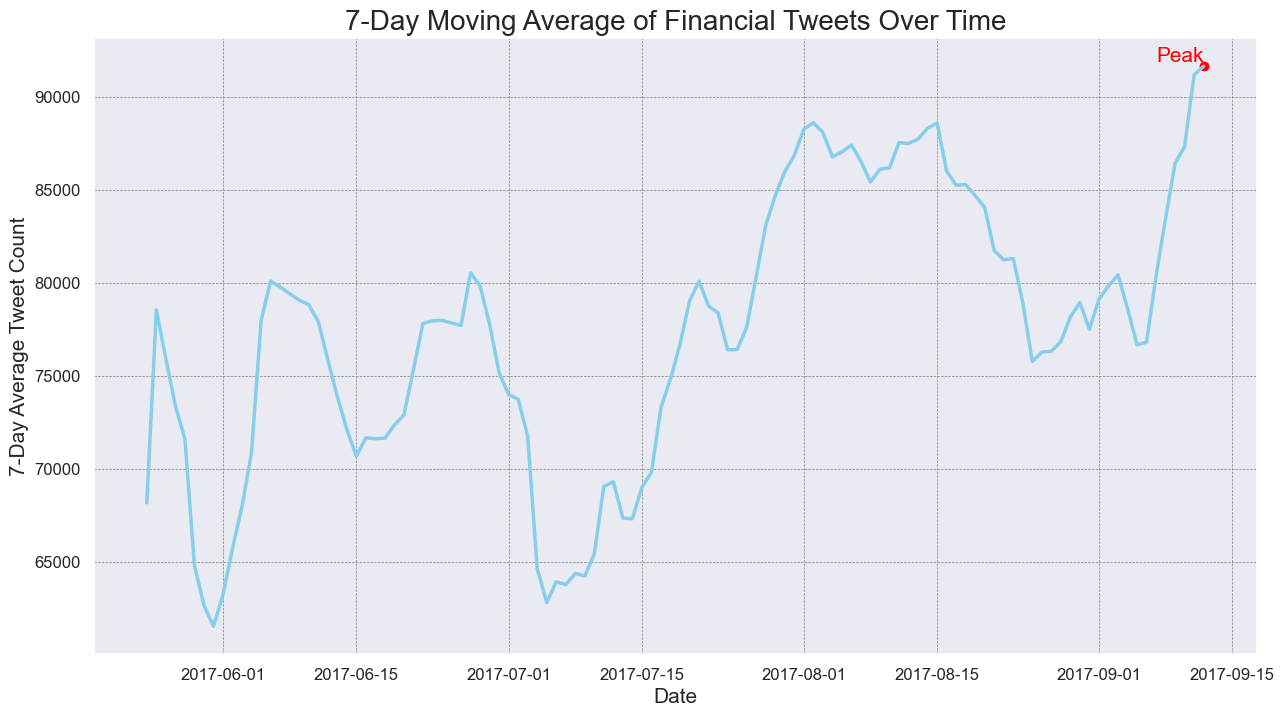
\includegraphics[width=1\textwidth]{P1.3.png}
    \caption{7-day average of all financial tweets over time}
    \label{fig:1.3}
\end{figure}

For this one I took on a 7-day moving average approach, just for
the sake of doing it.

\pagebreak

\subsection{Task 4}

\begin{qsolve}[Task]
    Statistics on distributions of retweets per tweets including 
    individual stocks (at least 2 chosen stocks) over time.
\end{qsolve}

\begin{figure}[h!]
    \centering
    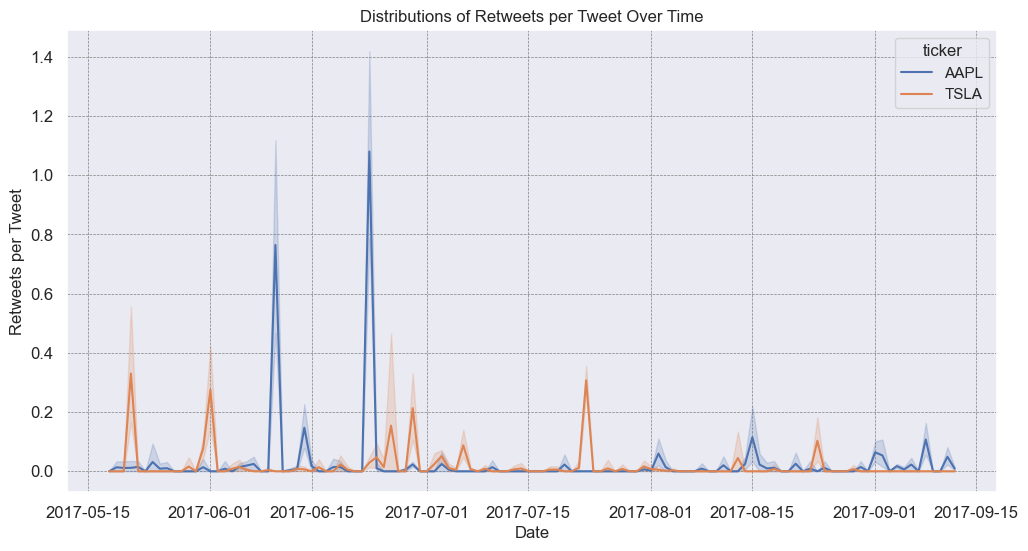
\includegraphics[width=1\textwidth]{P1.4.png}
    \caption{Distribution of retweets-per-tweet of \textbf{AAPL} and \textbf{TSLA} over time}
    \label{fig:1.4}
\end{figure}

I used Apple Inc. \textbf{(AAPL)} and Tesla Inc. \textbf{(TSLA)},
because I saw those in the demos and decided to use them for some reason.

\pagebreak

\subsection{Task 5}

\begin{qsolve}[Task]
    Statistics on most important financial information on 
    individual stocks (at least 2 chosen stocks) computed 
    solely from the financial information (not the tweets).
\end{qsolve}

\begin{figure}[h!]
    \centering
    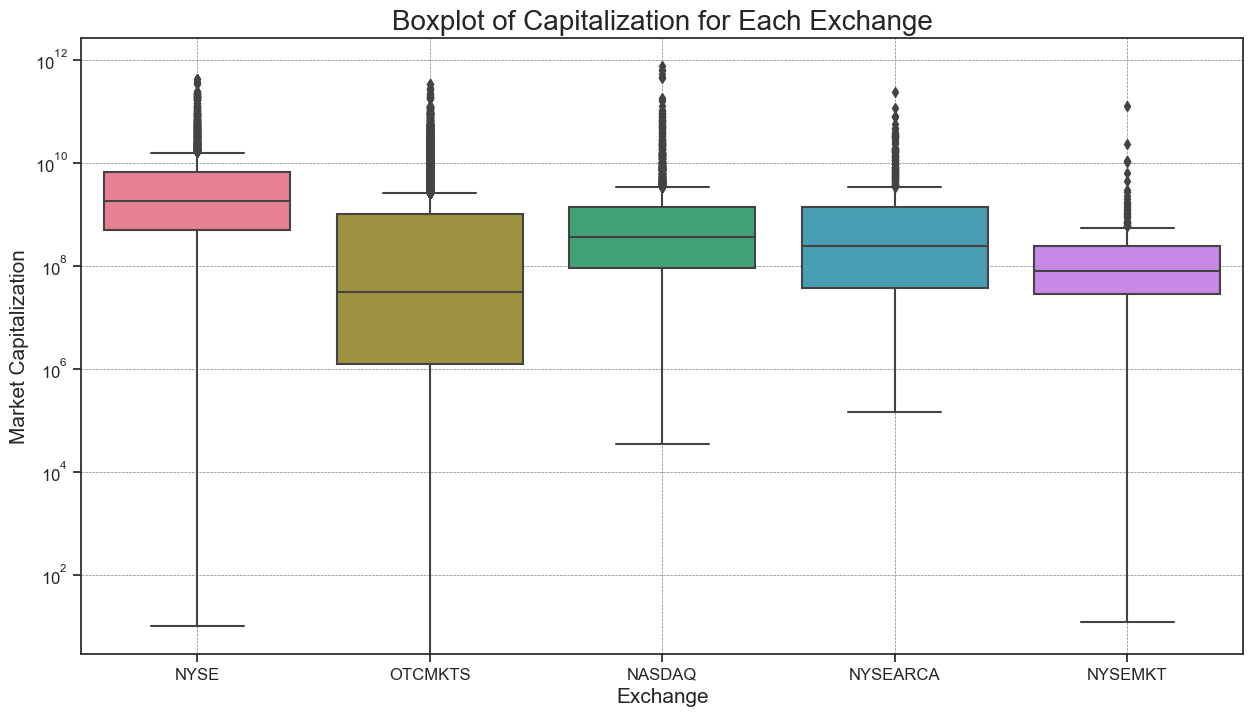
\includegraphics[width=1\textwidth]{P1.5.png}
    \caption{Box-plot of capitalizations per exchange (logarithmic)}
    \label{fig:1.5}
\end{figure}

The data for the box-plots was obtained from the 
`companies.csv' file.

\begin{figure}[h!]
    \centering
    \begin{subfigure}{.4\textwidth}
        \centering
        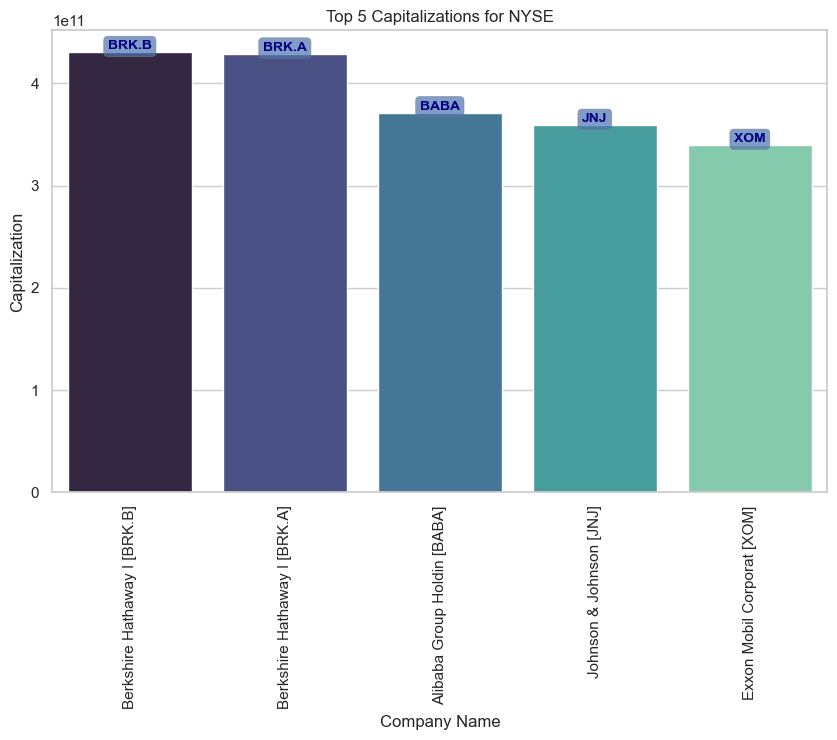
\includegraphics[width=.7\textwidth]{P1.5.1.png}
        \caption{NYSE}
        \label{fig:1.5.1}
    \end{subfigure}%
    \begin{subfigure}{.4\textwidth}
        \centering
        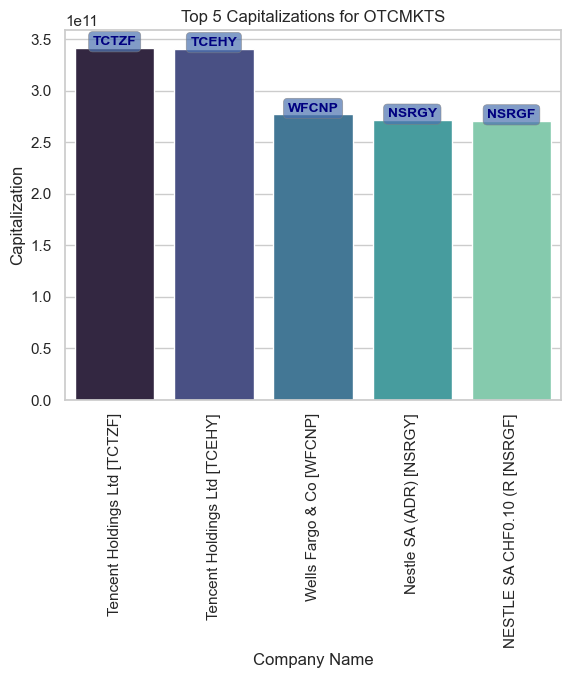
\includegraphics[width=.7\textwidth]{P1.5.2.png}
        \caption{OTCMKTS}
        \label{fig:1.5.2}
    \end{subfigure}

    \begin{subfigure}{.4\textwidth}
        \centering
        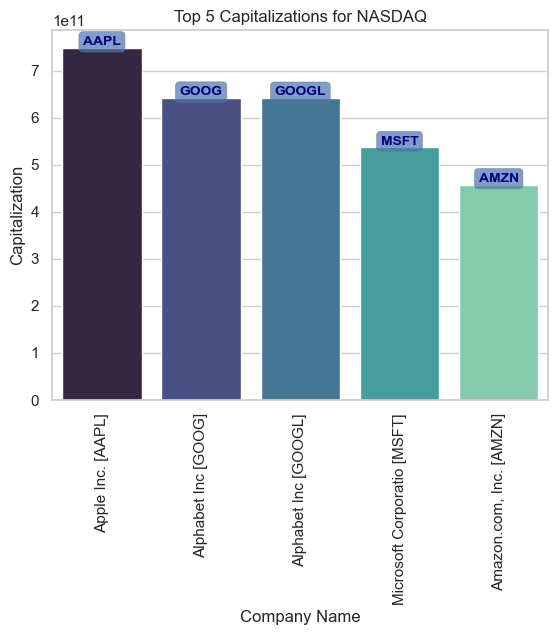
\includegraphics[width=.7\textwidth]{P1.5.3.png}
        \caption{NASDAQ}
        \label{fig:1.5.3}
    \end{subfigure}%
    \begin{subfigure}{.4\textwidth}
        \centering
        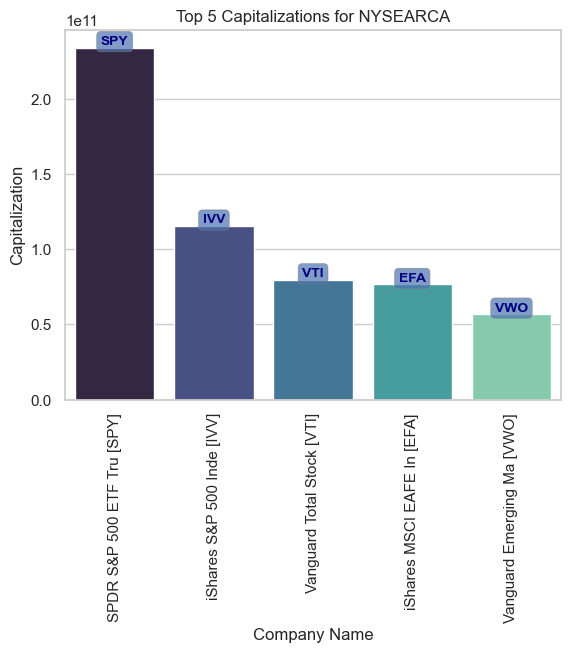
\includegraphics[width=.7\textwidth]{P1.5.4.png}
        \caption{NYSEARCA}
        \label{fig:1.5.4}
    \end{subfigure}
    \begin{subfigure}{.7\textwidth}
        \centering
        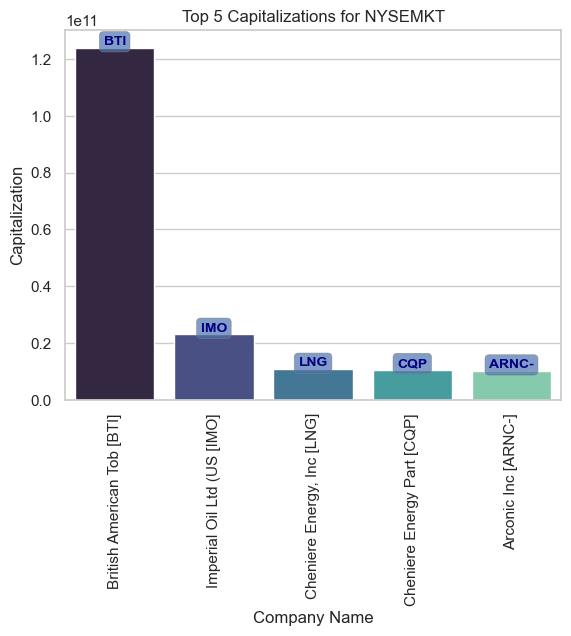
\includegraphics[width=.7\textwidth]{P1.5.5.png}
        \caption{NYSEMKT}
        \label{fig:1.5.5}
    \end{subfigure}
    \caption{Top 5 capitalizations for each exchange}
\end{figure}

\pagebreak

\subsection{Task 6}

\begin{qsolve}[Task]
    Time series movement directions through time for individual 
    stocks (at least 2). Choose companies you are familiar with. 
    Try to explain the reason behind these directions from real 
    world news.
\end{qsolve}

\begin{figure}[h!]
    \centering
    \begin{subfigure}{.4\textwidth}
        \centering
        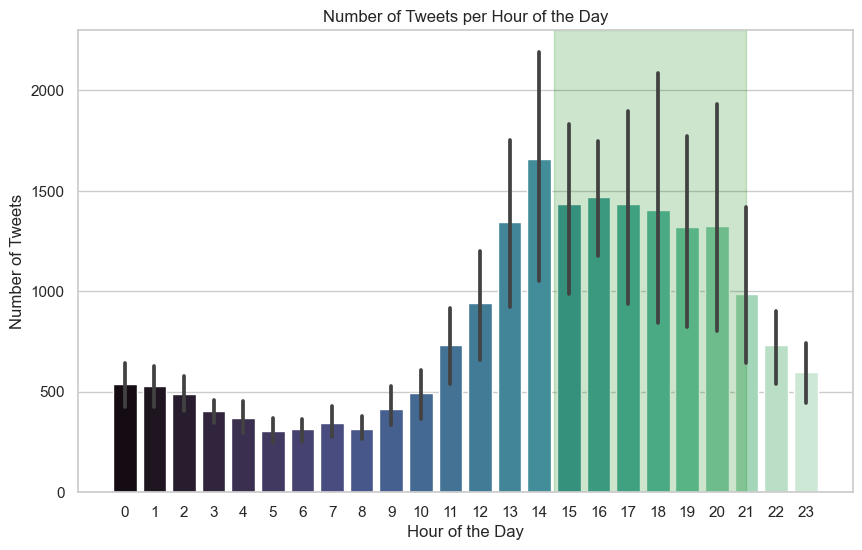
\includegraphics[width=.7\textwidth]{P1.6.3.png}
        \caption{Number of tweet per hour of the day}
        \label{fig:1.6.3}
    \end{subfigure}%
    \begin{subfigure}{.4\textwidth}
        \centering
        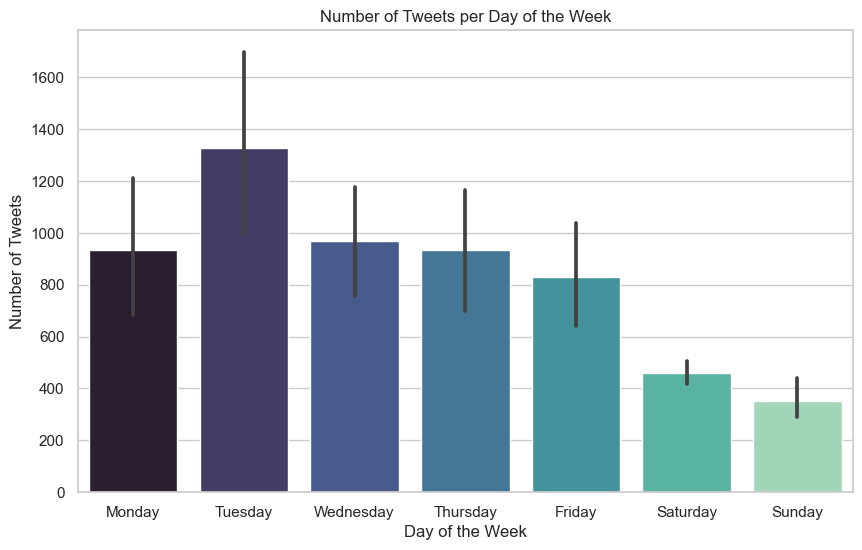
\includegraphics[width=.7\textwidth]{P1.6.2.png}
        \caption{Number of tweet per day of the week}
        \label{fig:1.6.2}
    \end{subfigure}
    \begin{subfigure}{.7\textwidth}
        \centering
        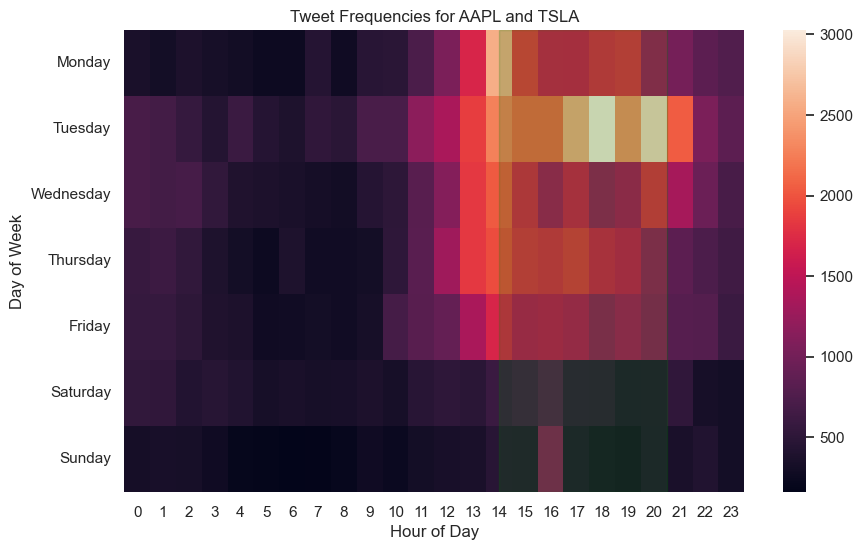
\includegraphics[width=.7\textwidth]{P1.6.1.png}
        \caption{Tweet frequencies per day of the week and hour of the day}
        \label{fig:1.6.1}
    \end{subfigure}
    \caption{Time series movement for number of tweets}
\end{figure}

\begin{itemize}
    \item In figure \textit{8.(a)}, we can see a peak at the trading hours 
    (highlighted green) and even an hour before trading hours. A psychological
    analysis may be that the traders will be checking tweeter an hour before trading
    to see how to market may be going, or maybe those interested in selling their shares
    may try to persuade buyers to buy their share of stock.

    \item In figure \textit{8.(b)}, we can see a drop on the days off (Saturday and Sunday).
    Tuesday seems to have a peak as well, but I lack knowledge of the
    market to be able to analyize why!

    \item In figure \textit{8.(c)}, we can see the joint distribution per day and week.
    The most frequent trading time is the trading hours in the working days.
    Tuesdays seem to be very heated (and I do not know why)!
\end{itemize}

\pagebreak

\subsection{Task 7}

\begin{qsolve}[Task]
    Co-occurence of various stocks in the same tweets.
\end{qsolve}

\begin{figure}[h!]
    \centering
    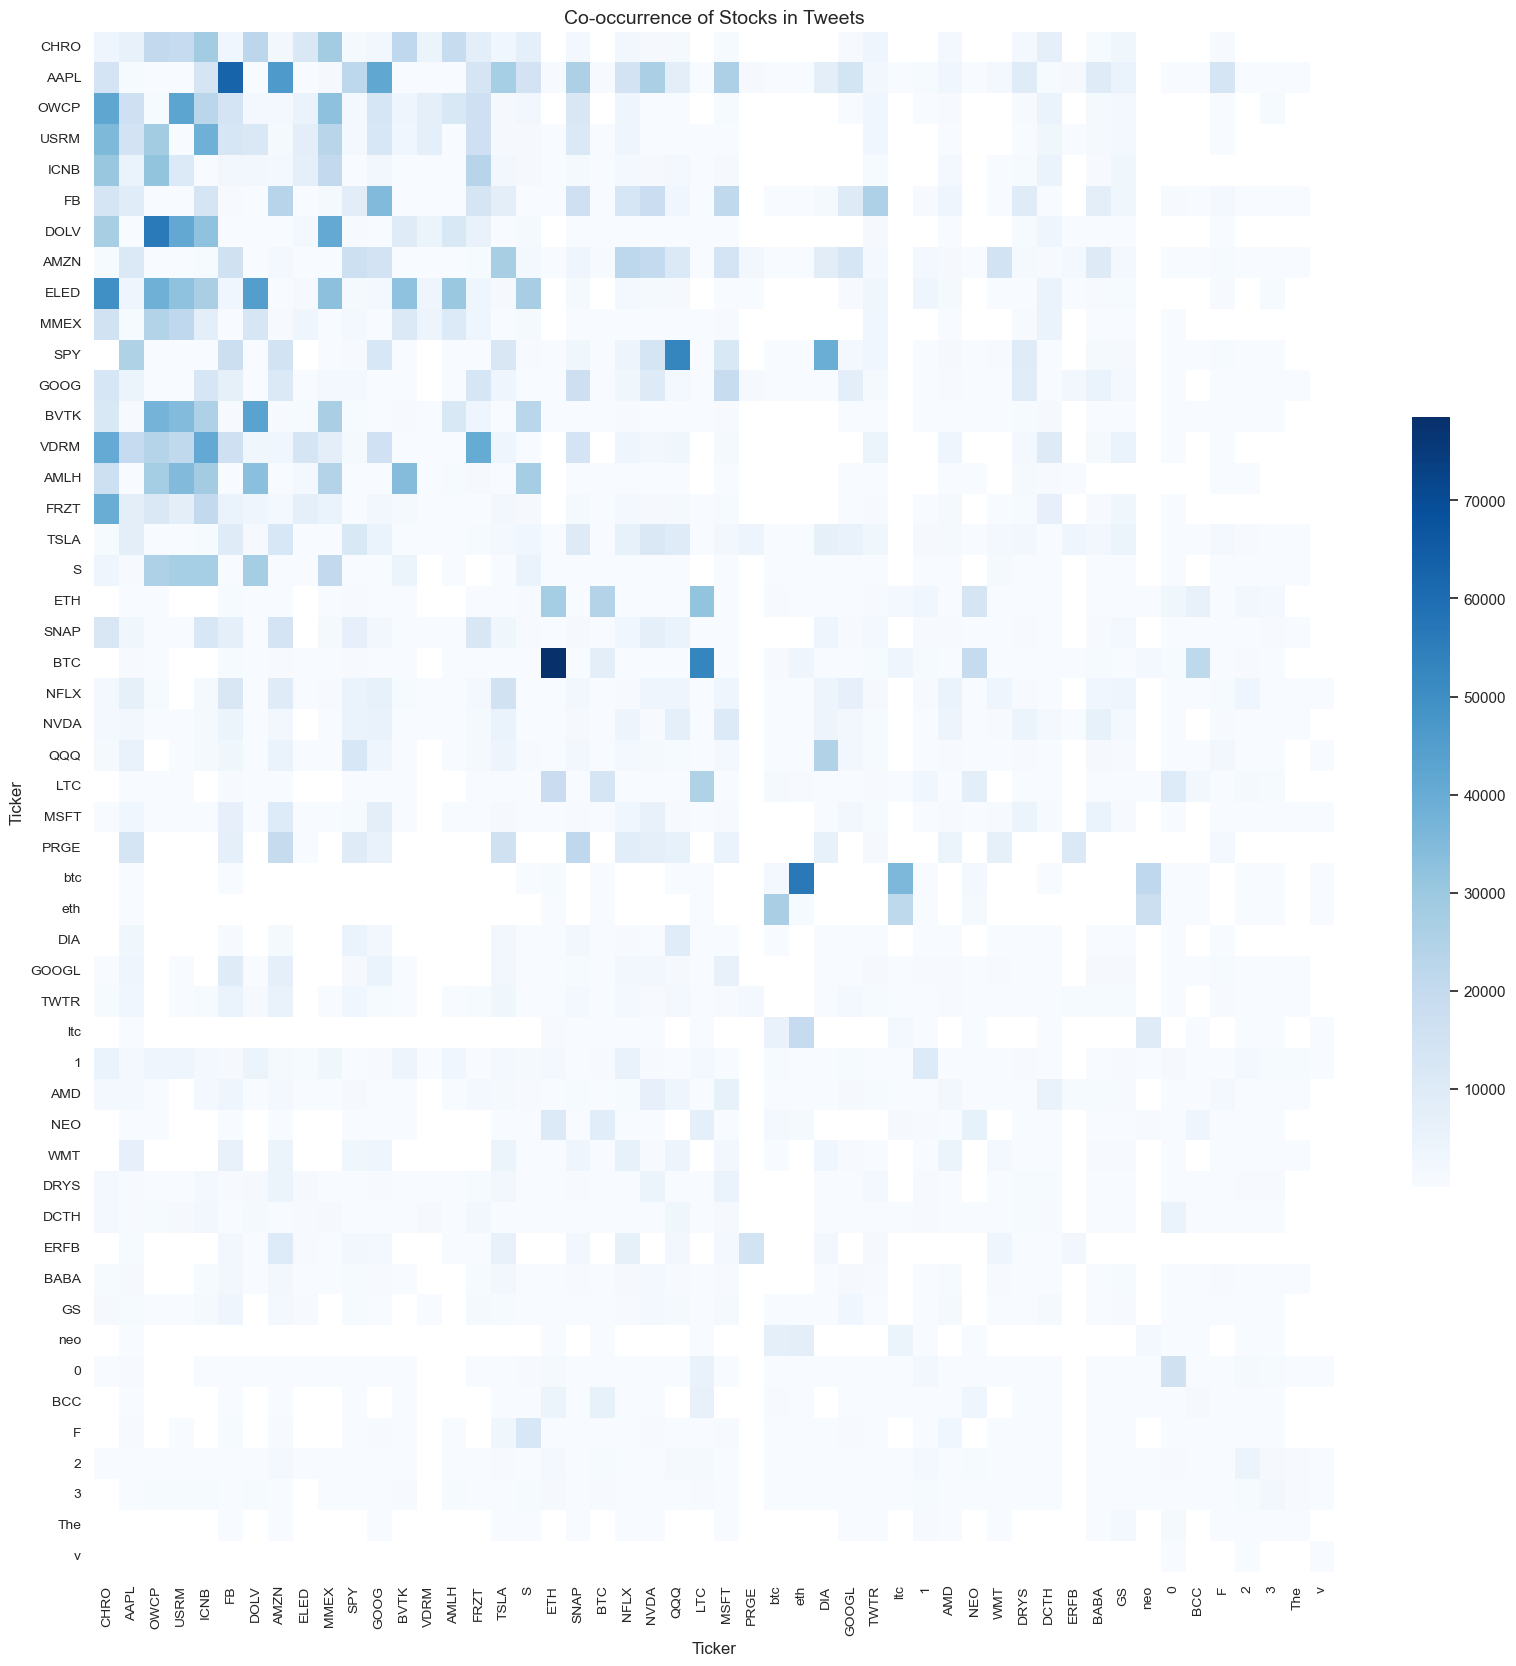
\includegraphics[width=1\textwidth]{P1.7.png}
    \caption{Co-occurence matrix of various stocks in the same tweet}
    \label{fig:1.7}
\end{figure}

The process is very time-consuming. I had to get the top 50 most 
common tickers to be able to computationally handle the task. It seems
\textbf{ETH} and \textbf{BTC} occur the most together. Another contestant
to that is \textbf{AAPL} and \textbf{FB}.

\section{Phase 2}
After reading the data and processing the time-series data, I was ready
to begin the training process. The problem was that the data size was
too huge for me to work with properly (as I tend to do the work with
trial and error), so I sampled the data and worked with a $N=100,000$
sample dataframe. All of the models were trained and evaluated this way.

I also had to use \textbf{Kaggle} for this Phase (and the next), because
my device did not have a usable GPU for training the models; I only had
a GPU there. Hopefully the file directories will make more sense when
you read the notebook now.

\subsection{Cleaning the data}

\begin{qsolve}[Task]
    Clean the data.
    \begin{itemize}
        \item Removing duplicate values and useless data (both columns and rows).
        \item Handling upper/lower case, etc.
    \end{itemize}
\end{qsolve}

First the links were removed. Then, the hashtags were separated 
from the text data, and punctuation was removed from the tweet.
All non-english characters were removed, and tokenized with the
stop-words removed. The stop-words were obtained from nltk.stop\_words.

\pagebreak

\subsection{Bag Of Words}

\subsubsection{Support Vector Machine (SVM)}

\begin{tabular}{lr}
    Train accuracy & 86.71\%\\
    Validation accuracy & 52.25\%\\
    Test accuracy & 51.77\%\\
\end{tabular}

\begin{figure}[h!]
    \centering
    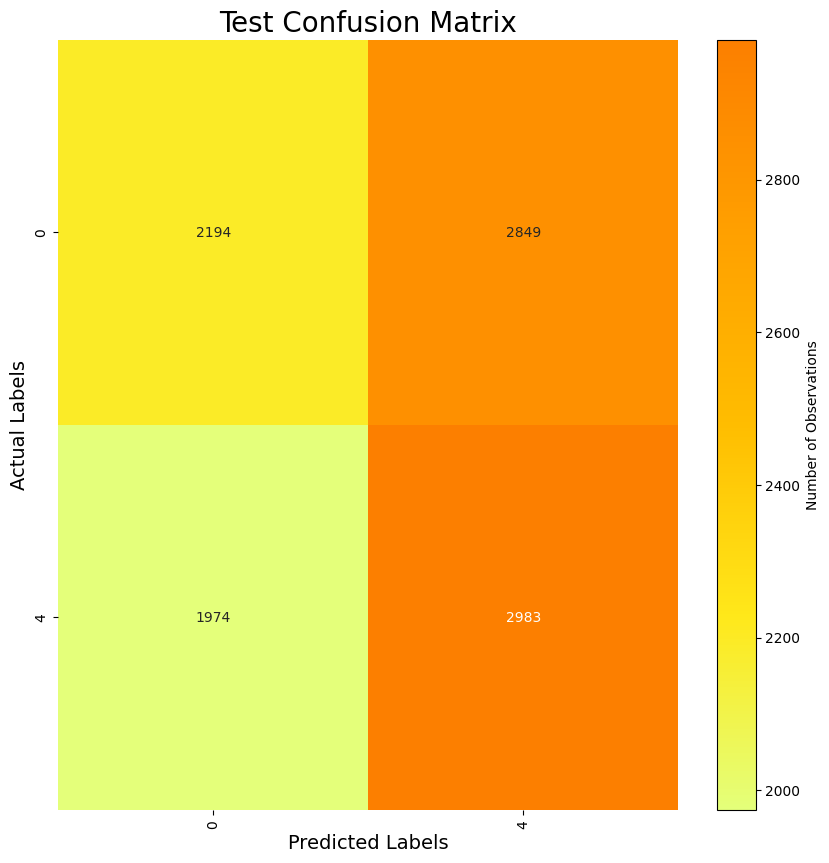
\includegraphics[width=.3\textwidth]{P2.BOW.1.png}
    \caption{SVM + BOW Confusion Matrix}
    \label{fig:2.BOW.1}
\end{figure}

\subsubsection{Random Forest}

\begin{tabular}{lr}
    Train accuracy & 96.43\%\\
    Validation accuracy & 52.12\%\\
    Test accuracy & 52.32\%\\
\end{tabular}

\begin{figure}[h!]
    \centering
    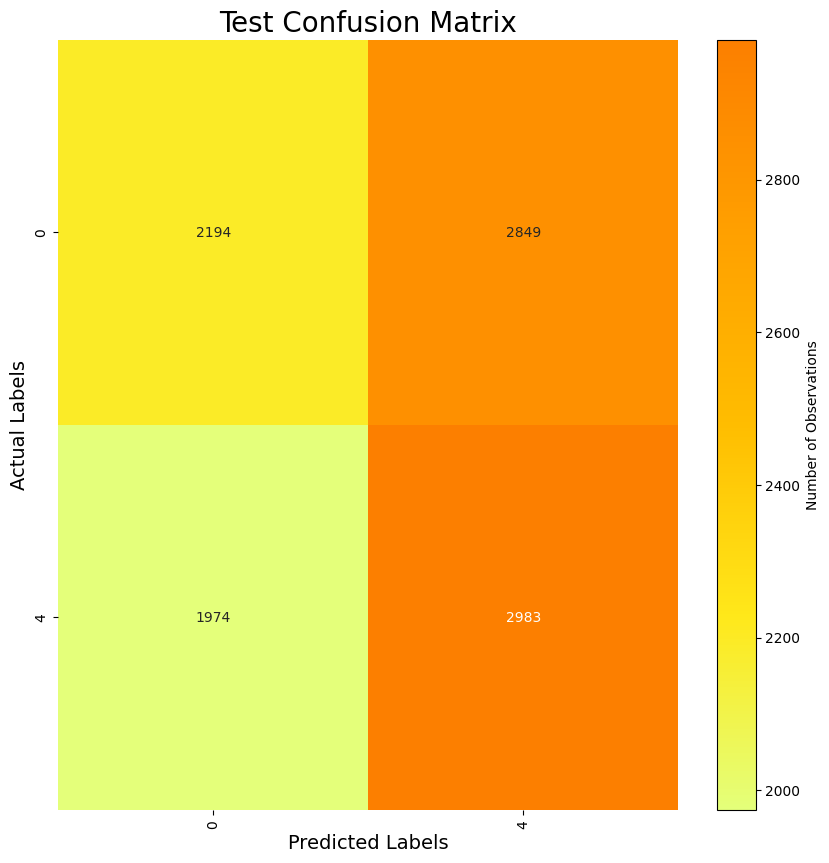
\includegraphics[width=.3\textwidth]{P2.BOW.1.png}
    \caption{Random Forest + BOW Confusion Matrix}
    \label{fig:2.BOW.2}
\end{figure}

The Random Forest already looks more promising, judging by the confusion matrices.
The main diagonal of the confusion matrix seems brighter. It seems
sentiment analysis is not linearly separable (what a surprise).

\subsection{TF-IDF}

\subsubsection{Support Vector Machine (SVM)}

\begin{tabular}{lr}
    Train accuracy & 94.92\%\\
    Validation accuracy & 77.62\%\\
    Test accuracy & 77.27\%\\
\end{tabular}

\begin{figure}[h!]
    \centering
    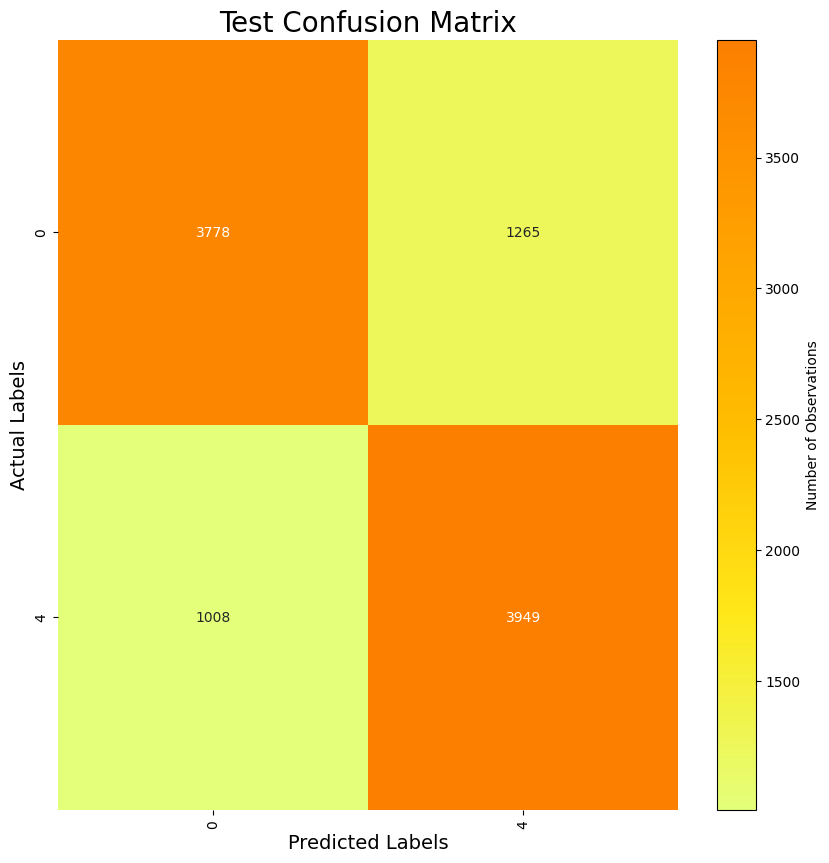
\includegraphics[width=.3\textwidth]{P2.TFIDF.1.png}
    \caption{SVM + TF-IDF Confusion Matrix}
    \label{fig:2.TDIDF.1}
\end{figure}

\subsubsection{Random Forest}

\begin{tabular}{lr}
    Train accuracy & 99.46\%\\
    Validation accuracy & 75.63\%\\
    Test accuracy & 75.54\%\\
\end{tabular}

\begin{figure}[h!]
    \centering
    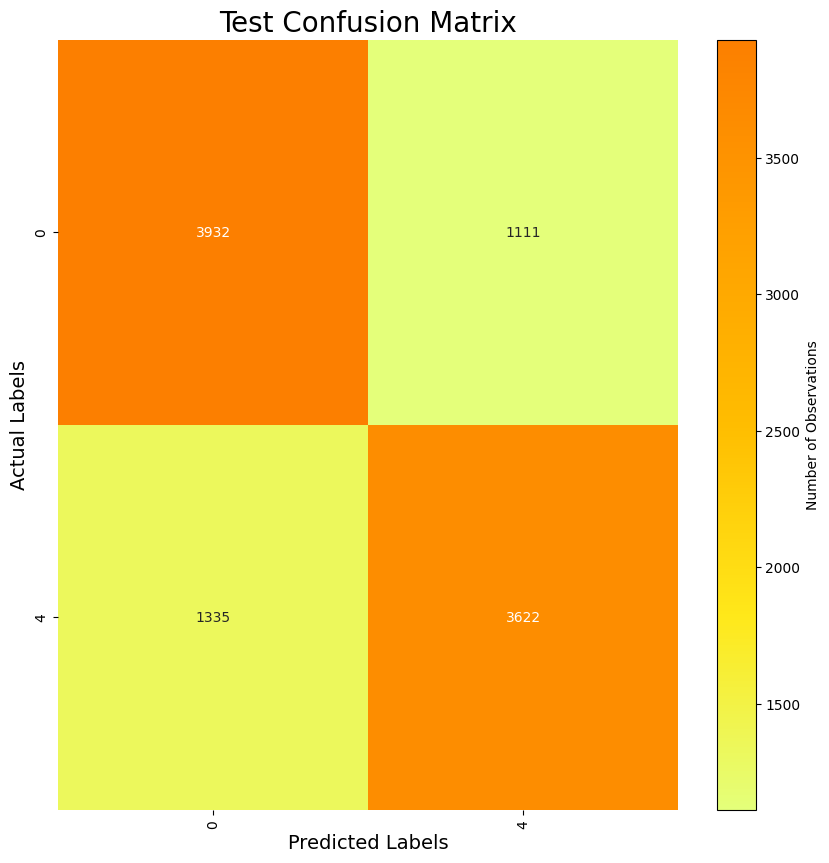
\includegraphics[width=.3\textwidth]{P2.TFIDF.2.png}
    \caption{Random Forest + TF-IDF Confusion Matrix}
    \label{fig:2.TFIDF.2}
\end{figure}

The Random Forest already looks more promising, judging by the confusion matrices, 
as the main diagonal of the confusion matrix seems brighter. TF-IDF
is already performing better than the BOW method.

\pagebreak

\subsection{SpaCy}
There is not much to say here really, except that I used the `textcat'
pipeline, already pre-prepared for our purpose (binary text-classification).

\begin{figure}[h!]
    \centering
    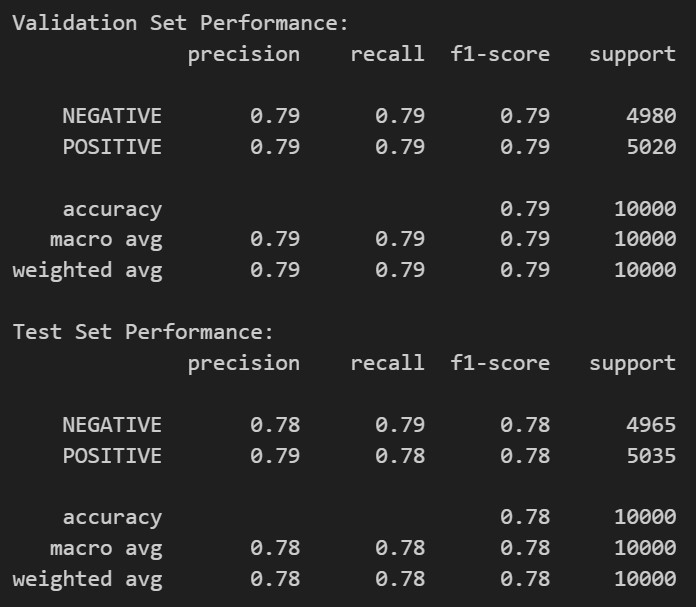
\includegraphics[width=.6\textwidth]{P2.SpaCy.jpg}
    \caption{SpaCy classifier metrics}
    \label{fig:P2.SpaCy}
\end{figure}

\subsection{Fine-tuning HuggingFace: Distil-BERT}

For the next section, I chose not to use the GPT API (because I did not
have enough time to calculate the token and chose to accept risk)
and instead used a fine-tuned version of the Distil-BERT model from 
HuggingFace. The reason I used SpaCy, was the fact that I did not like
having two BERT models for this project.

\begin{tabular}{lr}
    Train accuracy & 99.06\%\\
    Validation accuracy & 78.95\%\\
    Test accuracy & 77.85\%\\
\end{tabular}

\makeendpage
\end{document}